%% RiSE Latex Template - version 0.5
%%
%% RiSE's latex template for thesis and dissertations
%% http://risetemplate.sourceforge.net
%%
%% (c) 2012 Yguaratã Cerqueira Cavalcanti (yguarata@gmail.com)
%%          Vinicius Cardoso Garcia (vinicius.garcia@gmail.com)
%%
%% This document was initially based on UFPEThesis template, from Paulo Gustavo
%% S. Fonseca.
%%
%% ACKNOWLEDGEMENTS
%%
%% We would like to thanks the RiSE's researchers community, the 
%% students from Federal University of Pernambuco, and other users that have
%% been contributing to this projects with comments and patches.
%%
%% GENERAL INSTRUCTIONS
%%
%% We strongly recommend you to compile your documents using pdflatex command.
%% It is also recommend use the texlipse plugin for Eclipse to edit your documents.
%%
%% Options for \documentclass command:
%%         * Idiom
%%           pt   - Portguese (default)
%%           en   - English
%%
%%         * Text type
%%           bsc  - B.Sc. Thesis
%%           msc  - M.Sc. Thesis (default)
%%           qual - PHD qualification (not tested yet)
%%           prop - PHD proposal (not tested yet)
%%           phd  - PHD thesis
%%
%%         * Media
%%           scr  - to eletronic version (PDF) / see the users guide
%%
%%         * Pagination
%%           oneside - unique face press
%%           twoside - two faces press
%%
%%		   * Line spacing
%%           singlespacing  - the same as using \linespread{1}
%%           onehalfspacing - the same as using \linespread{1.3}
%%           doublespacing  - the same as using \linespread{1.6}
%%
%% Reference commands. Use the following commands to make references in your
%% text:
%%          \figref  -- for Figure reference
%%          \tabref  -- for Table reference
%%          \eqnref  -- for equation reference
%%          \chapref -- for chapter reference
%%          \secref  -- for section reference
%%          \appref  -- for appendix reference
%%          \axiref  -- for axiom reference
%%          \conjref -- for conjecture reference
%%          \defref  -- for definition reference
%%          \lemref  -- for lemma reference
%%          \theoref -- for theorem reference
%%          \corref  -- for corollary reference
%%          \propref -- for proprosition reference
%%          \pgref   -- for page reference
%%4
%%          Example: See \chapref{chap:introduction}. It will produce 
%%                   'See Chapter 1', in case of English language.

\documentclass[pt,oneside,onehalfspacing,bsc]{risethesis}

\usepackage{natbib}
\usepackage{babel}
\usepackage{supertabular}
\usepackage{microtype}
\usepackage{lscape}
\usepackage{mathtools}
\usepackage{amsmath}
\usepackage{multirow}
\usepackage{tikz}
\usepackage{float}
\usepackage{url}
\usepackage{enumitem}
\usepackage{listings}


%% Aumenta a margem entre o label e as tabelas
% \usepackage{caption}
% \captionsetup[table]{skip=8pt}

%% Label at the bottom
\lstset{
	captionpos=b,
	basicstyle=\ttfamily,
	columns=fullflexible,
	frame=single,
	breaklines=true,
	postbreak=\mbox{\textcolor{red}{$\hookrightarrow$}\space}
}

\DeclarePairedDelimiter\abs{\lvert}{\rvert}%
\DeclarePairedDelimiter\norm{\lVert}{\rVert}%
\newcommand{\me}{\mathrm{e}}

% Swap the definition of \abs* and \norm*, so that \abs
% and \norm resizes the size of the brackets, and the 
% starred version does not.
\makeatletter
\let\oldabs\abs
\def\abs{\@ifstar{\oldabs}{\oldabs*}}
%
\let\oldnorm\norm
\def\norm{\@ifstar{\oldnorm}{\oldnorm*}}
\makeatother


%% Change the following pdf author attribute name to your name.
\usepackage[linkcolor=blue,citecolor=blue,urlcolor=blue,colorlinks,pdfpagelabels,pdftitle={Monografia de Daniel Santos Peixoto},pdfauthor={Daniel Santos Peixoto}]{hyperref}

\address{SALVADOR}

\universitypt{Universidade Federal da Bahia}

\departmentpt{Departamento de Ciência da Computação}

\programpt{}

\majorfieldpt{Ciência da Computação}
\majorfielden{Computer Science}

\title{Um Sistema de Recomendação Semântico Baseado em Conteúdo}
\date{Setembro/2018}

\author{Daniel Santos Peixoto}
\adviser{Frederico Araújo Durão}

\begin{document}

\frontmatter
\frontpage
\presentationpage

\begin{epigraph}[]{William Ernest Henley}
It matters not how strait the gate, how charged with punishments the scroll, I am the master of my fate, I am the captain of my soul
\end{epigraph}

\resumo
Neste trabalho abordamos os meios mais eficientes para obter resultados satisfatórios em buscas realizadas em fóruns de perguntas e resposta. Neste cenário precisamos, além de considerar semelhança entre a busca e os objetos contidos no universo de busca, precisamos garantir que a solução é viável em tempo e recursos, e também verificar se os itens encontrados são capazes de solucionar o problema inquerido na busca. Pensando nisso, propomos um meio que leva em consideração metadados contidos na maior parte dos fóruns de perguntas e respostas e usamos uma ferramenta que cumpre a limitação de tempo e permite a configuração de busca desejada. 

\begin{keywords}
search, forums, crowdsourced knowledge, qa
\end{keywords}
\abstract
TODO

\begin{keywords}
search, forums, crowdsourced knowledge, qa
\end{keywords}

\tableofcontents
\listoffigures
\listoftables

% List of acronyms
% Acronyms manual: http://linorg.usp.br/CTAN/macros/latex/contrib/acronym/acronym.pdf
\listofacronyms
\begin{acronym}[ACRONYM] 

\acro{NFC} {Need For Cognition}
\acro{API} {Application Programming Interface}
\acro{SR} {Sistema de Recomendação}
\acro{CF} {Collaborative Filtering}
\acro{CBF} {Content Based Filtering}
\acro{RMSE} {Root Mean Square Error}
\acro{WWW} {World Wide Web}
\acro{W3C} {World Wide Web Consortium}
\acro{SQL} {Structured Query Language}
\acro{NLP} {Natural Language Processing}
\acro{TFIDF} {Term Frequency Inverse Document Frequency}

% Bruno
\acro{RI} {Recuperação de Informação}
\acro{RD} {Recuperação de Dados}
\acro{LSI} {Latent Semantic Indexing}
    
\end{acronym}

% List of listings
%\lstlistoflistings

\mainmatter
%\setcounter{page}{21}
\chapter{Introdução}
\label{cap:introduction}

\begin{quotation}[]{Yoko Ono}
The computer is my favourite invention. I feel lucky to be part of the global village. I don't mean to brag, but I'm so fast with technology. People think it all seems too much, but we'll get used to it. I'm sure it all seemed too much when we were learning to walk.
\end{quotation}

A popularização da Internet permitiu que a obtenção e geração de conhecimento também se tornasse acessível à uma maior parte da população. Temos mais de 3.8 bilhões de usuários \cite{dataneversleeps6}, geramos 2.5 petabytes todos os dias \cite{dataperday}, as enciclopédias foram substituídas por wikis, aulas e cursos já estão migrando para serviços de streaming e as discussões saíram dos espaços físicos para os fóruns. Além disso, o conhecimento agora é mais democrático, muito mais pessoas podem produzir conteúdo, são mais de 600 edições de páginas na Wikipédia\footnote{https://www.wikipedia.org/} por minuto \cite{dataneversleeps5}, não somente grandes empresas ou acadêmicos, e qualquer um com uma rede de Internet pode consumir esse conteúdo criado. 

Platão, famoso filósofo grego, criou um método chamado dialética, onde, junto com sua academia, buscava estabelecer a verdade por meio de discussões sobre dúvidas e problemas. A dialética contrasta com a didática, onde se propõe que um dos interlocutores seja o único à transmitir à informação, desfavorecendo o debate. Da mesma forma, por meio dos fóruns, o conteúdo é orientado às perguntas em vez da exposição do conteúdo em si, tornando aos métodos de ensino indicados por Platão. 

Existem diversos tipos de fóruns na Internet, alguns mais conhecidos como Yahoo Respostas\footnote{https://www.answers.yahoo.com/}, StackOverflow\footnote{https://www.stackoverflow.com/}, AskUbuntu\footnote{https://www.askubuntu.coms/}, etc e também alguns com domínios específicos para comunidades, que podem falar sobre animes, filmes, música, empreendedorismo e etc. Os grandes fóruns, normalmente contam com equipes especializadas para seu funcionamento, entretanto os pequenos, são normalmente criados em plataformas que também os hospedam, como é o caso da Fandom\footnote{https://www.fandom.com/}, que permite que usuários hospedem fóruns de entretenimento gratuitamente. Graças à eles, aqueles que tem perguntas, possuem meios para interagir com os que detêm conhecimento de um determinado domínio, além de compartilhar essa interação com o resto da comunidade, que está ao redor de todo o globo.

Graças aos mecanismos de interação do usuário com a informação, é possível se verificar a relevância de uma dada informação. O StackOverflow\footnote{https://www.stackoverflow.com/} usa dessa estratégia para que as respostas possam ser validadas ou não pela comunidade. Por meio de votos positivos e negativos, comentários, avaliação do próprio autor do tópico, a comunidade pode expressar sua opinião sobre as respostas ofertadas.

Com um número tão grande de informação, os usuários precisam de ajuda pra encontrar a informação desejada, com este problema, surgiram os buscadores. Buscadores com Google\footnote{https://www.google.com/}, Bing\footnote{https://www.bing.com/} já estão disponíveis há bastante tempo, só o Google, realiza mais de 3.5 bilhões de buscas todos os dias \cite{googlesearch}, porém cada vez mais encontramos buscadores específicos para determinados conteúdos, como é o caso do Google Scholar\footnote{https://www.scholar.google.com/}, YouTube\footnote{https://www.youtube.com/}, Buscapé\footnote{https://www.buscape.com.br/}, etc. Para resolver o problema do usuário, se tornou necessária a criação de buscadores para fóruns.

%Os fóruns de perguntas e respostas funcionam com usuários que realizam perguntas e outros respondendo à estas perguntas, essa interação é avaliada pela comunidade, que verifica a clareza e a qualidade não só das respostas, mas também das perguntas, pois com uma pergunta escrita de forma clara, se torna mais fácil para se verificar a real intenção do autor.

\section{Motivação}
Cerca de 80\% à 84\% das buscas no Google já foram feitas anteriormente \cite{googleexplained}, isso mostra como a reincidência de buscas é algo comum. Da mesma forma, tópicos em fóruns tendem a se repetir. É muito importante que um buscador de fóruns traga bons resultados. Se um usuário não possui sua dúvida sanada por meio do histórico já existente, ele deve criar um novo tópico para esse banco de dados, o que implicará, quando essa resposta já existe, em um retrabalho para a discussão nesse tópico e um aumento desnecessário do problema, já que agora temos mais um item no banco de dados.

Por outro lado, técnicas que demandem muito esforço podem ser inviabilizadas pela restrição do tempo, já que se espera que os resultados sejam entregues em questão de segundos. Para uma única busca, o Google usa mil computadores em 0.2 segundos para trazer uma resposta \cite{buildinggoogle}, mas o que vale para o Google, não necessariamente vale para a realidade de outros buscadores. Por esta razão, precisamos trazer soluções que sejam viáveis para os pequenos fóruns que dependem de uma plataforma pública para hospedagem, permitindo que as plataformas possam implementar essa ferramenta, sem muito custo adicional.

Devido à tamanha complexidade e a falta de ferramentas disponíveis, não somente os fóruns pequenos, mas também as grandes plataformas e os grandes fóruns, abrem mão de um serviço de busca eficiente. 
\section{Problema}
O problema que esse trabalho visa resolver é a baixa precisão nos buscadores de fóruns diante de um cenário em que os são recursos limitados. O seguinte estudo verifica meios para retornar bons resultados ainda que não se haja tanto poder computacional e/ou grandes equipes de desenvolvimento, de forma que, a solução deva ser simples e eficiente.

Com bilhões de informações disponíveis, precisamos usar filtros para encontrar a informação desejada. Para isso, precisamos verificar a relevância e a utilidade que esta informação possui, pois nem toda informação recebida é necessariamente verdade ou capaz de solucionar o problema do usuário. Porém, esta mesma tarefa tem que ser executada em tempo hábil para se prover uma resposta satisfatória para o usuário, o que é outro problema já que consideramos um número massivo de dados. 

Ainda que tenhamos metadados, é preciso entender o valor que estes trazem para a busca. Informações como datas, feedbacks positivos e interação com conteúdo podem ter influências diferentes dependendo do domínio utilizado, já que alguns conteúdos podem ser desvalorizados com o passar do tempo e outros perdurarem, da mesma forma, algumas perguntas por serem mais frequentemente encontradas podem ter a tendência de ter mais interações que outras, o que pode prejudicar as perguntas que não ocorrem tão frequentemente.

Assim, considerando que o público-alvo tem um grande volume de dados e recursos limitados é necessário descartar opções muito custosas.

\section{Objetivos da Solução Proposta}
O objetivo desse trabalho é trazer conteúdos já existentes nos fóruns que podem possivelmente resolver o anseio do usuário expresso em uma busca de maneira rápida e não muito custosa. Tendo como objetivos específicos:

\begin{itemize}
    \item Revisão da literatura existente de Recuperação da Informação
    \item Recuperar tópicos já existentes que sejam relevantes à busca do usuário.
    \item Propor um método eficiente para avaliar a relevância do conteúdo para uma dada busca.
    \item Realizar uma avaliação experimental a fim de verificar-se a qualidade das buscas.
\end{itemize}

\section{Estrutura}

<Resumo do que será visto nos próximos capítulos>
\chapter{Fóruns}
\label{cap:forums}

\begin{quotation}[]{Yoko Ono}
The computer is my favourite invention. I feel lucky to be part of the global village. I don't mean to brag, but I'm so fast with technology. People think it all seems too much, but we'll get used to it. I'm sure it all seemed too much when we were learning to walk.
\end{quotation}

De acordo com o dicionário, fóruns são um lugar ou meio onde ideias e visões sobre um particular assunto podem ser trocadas. Ao aprofundar mais no presente problema, fóruns de perguntas e respostas são lugares ou meios onde perguntas podem ser feitas e ideias e visões possam ser usadas como resposta. 
\section{Histórico}
Um dos primeiros fóruns de perguntas e respostas a surgir foi o Answer Point, disponibilizado pelo Ask Jeeves na década de 90. Seu slogan era: "Answer Point é o lugar onde você pode fazer e responder perguntas. Tem uma dúvida? Publique-a! Sabe a resposta? Publique-a!" \cite{websearchhistory}.

 De acordo com Jim Lanzone, vice-presidente sênior do AskJeeves, a maior dificuldade era pra incentivar usuários à responder. Com poucas questões respondidas, Jim Lanzone defende a utilidade dos engenhos de busca, pois a maioria das buscas são únicas, ainda que a relevância não seja perfeita, é possível trazer resultados amplos \cite{websearchhistory}. Além disso, esperar por uma resposta é conflitante com o que o usuário mais precisa, velocidade. 

A Ask Jeeves possuia outros produtos além do AnswerPoint, o seu principal era o Ask.com, um buscador concorrente ao do Google. Segundo Jim Lanzone, a empresa decidiu focar em outros aspectos do seu buscador e descontinou o projeto do AnswerPoint \cite{websearchhistory}.

Na mesma semana do fechamento do Answer Point, foi lançado o Google Answers \cite{googleanswerswiki}. O Google Answers era um serviço que permitia que as pessoas submetessem perguntas e oferecessem um pagamento por sua resposta, este pagamento podia variar de 2,50 dólares até 200.50 dólares. Entretanto, também era possível ver respostas para outras perguntas já respondidas sem efetuar pagamento. Seu fracasso, dentre outros motivos, foi decorrente principalmente do surgimento de serviços de perguntas e respostas gratuitos.

O Yahoo Respostas foi criado pela empresa Yahoo no ano 2005. Foi um dos primeiros a implementar o crowdsourcing \footnote{Crowdsourcing é um modelo de produção que conta com a força do coletivo para desenvolver soluções.} com sucesso. A empresa implementou um sistemas de pontos para incentivar os usuários à responder perguntas. Com esses pontos, os usuários possuem mais acesso à plataforma, os permitindo publicar mais questões e respostas. A pontuação é atribuída pelo autor da pergunta e também pela comunidade que pode manifestar sua opinião \cite{yahooanswerswiki}.

Em 2004, Tim O'Reilly cunhou o termo de Web 2.0, ele se referia à uma web participativa, com conteúdo produzido pelos próprios internautas \cite{webtransition}. Atualmente, com a popularização dos dispositivos móveis, facilitou-se o acesso do usuário à rede e, consequentemente, sua participação. Os usuários passaram a confiar e depender cada vez mais desses meios de interação, dentre eles, os fóruns, o que tornou necessária uma web mais organizada, chamada de Web 3.0 por John Markoff. Na Web 3.0, a informação é estruturada não somente em meios inteligíveis por humanos, mas também por máquinas. Por meio das máquinas, se torna possível um acesso mais rápido à informação. É um uso mais inteligente do conteúdo já disponibilizado online.
\section{Exemplos}
Com o crescimento exponencial da internet, houve espaço para novos fóruns crescerem e se desenvolverem em nichos diferentes. São estes alguns exemplos relevantes.
\subsection{Quora}
Quora\footnote{https://quora.com/} é um espaço pra perguntas e respostas para qualquer domínio. A empresa foi criada por Adam D'Angelo e Charlie Cheever e disponibilizada ao público em 2010.

O fórum Quora tornou-se uma opção mais usada pelos usuários devido à um uso mais consciente dos fóruns, onde perguntas devem ser mais bem elaboradas e bem estruturadas. Perguntas que não são adequadas são reportadas e removidas da plataforma.

Isso tornou-se necessário pois o Yahoo Respostas estava se tornando muito poluído com perguntas vagas \cite{quoravsyahoo}, como a de estudantes para responder tarefas de casa e com respostas sem sentido, às vezes apenas com "Eu não sei", que serviam para que ainda assim ganhassem pontos na plataforma.

Graças à esta nova visão, usuários da plataforma têm um acesso facilitado às perguntas de seu interesse e menos conteúdo duplicado, além de que agora a plataforma consegue melhor recomendar perguntas aos usuários que podem a responder.
\subsection{StackOverflow}
Criado por Jeff Atwood e Joel Spolsky em 2008. Jeff era um desenvolvedor e possuia um blog chamado de Coding Horror\footnote{https://blog.codinghorror.com/} onde abordava temas relacionados à programação \cite{codinghorror}. No mês de julho de 2008, quando foi criado, Jeff limitou o acesso para aqueles que eram assinantes do blog e no mês de setembro tornou público o acesso.

O sucesso da plataforma foi tamanho que permitiu que crescesse para um conglomerado de fóruns de perguntas e respostas sobre vários outros tópicos, conhecido com StackExchange, onde são mantidos o próprio StackOverflow, AskUbuntu, SuperUser e mais de 150 outros. Atualmente, a plataforma possui mais de 17 milhões de perguntas.

\section{Usos Mercadológicos}

\subsection{Vendas Direcionadas}
Uma das formas mais comuns de se gerar renda é através de anúncios direcionados. Um dos que usam essa abordagem é o Quora, que hoje é avaliado em mais de 1,8 bilhão de dólares \cite{quorarevenuemodel}.

\subsection{Recrutamento}
Ao responder perguntas, os usuários criam notoriedade pra si. O StackExchange usa essa vantagem tanto para estimular usuários para responder perguntas, quanto pra identificar potenciais para determinadas vagas.

Apresentadas em forma de anúncio, vagas são ofertadas para os usuários de acordo com o seu perfil na plataforma. Da mesma forma, os recrutadores tem acesso à informações mais detalhadas dos candidatos, graças à participação dos mesmos, que os garante reconhecimento na comunidade e troféus fictícios na plataforma.

%\section{Projetos}
%\subsection{Question Answering}
%\subsection{Identificação de perguntas duplicadas}
%\subsection{Recuperação de Perguntas}
\section{Sumário}
\chapter{Recuperação da Informação}
\label{cap:informationretrieval}

\begin{quotation}[]{Yoko Ono}
The computer is my favourite invention. I feel lucky to be part of the global village. I don't mean to brag, but I'm so fast with technology. People think it all seems too much, but we'll get used to it. I'm sure it all seemed too much when we were learning to walk.
\end{quotation}

A necessidade das pessoas de encontrar informação tem crescido bastante e tem se tornado uma prática de seu cotidiano. As informações devem ser precisas e estar disponíveis quase que imediatamente. Este capítulo fornece uma visão geral sobre Recuperação de Informação, a diferença entre recuperar uma informação e recuperar um dado e as técnicas utilizadas nas buscas.

\section{Introdução}

Nos tempos atuais, com o crescimento das bibliotecas virtuais e trocas eletrônicas de informações, há uma necessidade clara no melhoramento das técnicas de busca de informação. A gigantesca quantidade de informação e o tempo hábil do usuário para esperar por esses resultados são os fatores mais determinantes. 

Tendo como foco a melhoria na qual os dados são encontrados e celeridade em que são exibidas para o usuário, a indexação é uma das principais técnicas utilizadas em conjunto com outros algoritmos complexos \cite{Fred2008}.

Buscar informações, embora pareça uma atividade simples, é um processo muito impreciso. É esperado que o usuário possua uma noção vaga ao tentar buscar por uma informação, uma vez que não há uma interface direta que interprete exatamente às demandas do usuário e o resultado depende dos dados inicialmente fornecidos. Portanto, a interface deve ajudar o usuário na compreensão e expressão das necessidades de informação da melhor forma possível. Na formulação de suas consultas, fazendo a seleção da informação dentro de um conjunto de documentos, entendendo os resultados da pesquisa e acompanhar o progresso de suas buscas \cite{Baeza-Yates1999}.

\section{Recuperação de Informação versus Recuperação de Dados}

Uma série de características distinguem sistemas de Recuperação de Informação (\ac{RI}) de outras ferramentas de acesso à dados. Um sistema de \ac{RI} não extrai informações dos documentos acessados e normalmente também não processa as informações contidas nesses objetos. Isso separa os sistemas de RI de sistemas baseados no conhecimento, como sistemas especialistas. Essas ferramentas baseadas no conhecimento dependem fortemente de uma representação pré-definida de um domínio. Este conhecimento é geralmente utilizado para inferir, manipular ou categorizar informações através de dados. Diferente disso, os sistemas de Recuperação de Informação são usados para direcionar o usuário para documentos que possam ajudar a satisfazer suas necessidades de informação \citep{Ruthven2003}.

Recuperação de Dados (\ac{RD}) tem o propósito de encontrar dados que casam perfeitamente com a consulta, enquanto recuperação de informação visa encontrar os dados que possuam no mínimo alguma similaridade. Consequentemente, recuperação de dados é mais sensível à erros, considerando que um único documento errado retornando dentro de uma lista de outros milhares corretos, é uma falha total da busca. Por outro lado, recuperação de informação pode ser imprecisa e erros eventuais não compromete completamente o resultado da busca. Isso acontece porque recuperação de informação geralmente lida com textos semi-estruturados de linguagem natural, que pode ser semanticamente ambíguo enquanto recuperação de dados, procura por dados dentro de um ambiente estruturado, como por exemplo, um banco de dados relacional \cite{Fred2008}.

\begin{table}[htb]
	\centering
	\caption{Diferença entre sistemas \ac{RI} e \ac{RD}.}
	\label{tab:RIxRD}
	\begin{tabular}{|m{7cm} | m{2cm} | m{2cm} |}

		\hline
		
		\multicolumn{1}{|c|}{\bfseries Características / Métodos } & \multicolumn{1}{c|}{\bfseries RI} & \multicolumn{1}{c|}{\bfseries RD}\\ \hline
		Combinação exata   					&		&	x 	\\ \hline
		Alta sensibilidade a erros   			&		&	x  	\\ \hline
		Tratamento semântico   				&	x 	&	 	\\ \hline
		Busca em dados não estruturados   	&	x 	&	 	\\ \hline
		Inferência Dedutiva  					&		&	x  	\\ \hline
		Inferência Indutiva   					&	x 	&	 	\\ \hline
		Consulta de sintaxe controlada   		&		&	x 	\\ \hline
		Consulta com linguagem Natural   	&	x 	&	 	\\ \hline
		Mais utilizado em meios acadêmicos   &	x 	&	 	\\ \hline
		Comum em Produtos Comerciais   	&		&	x 	\\ \hline
		
	\end{tabular}
\end{table}

Ainda segundo \cite{Fred2008}, o usuário que utiliza um sistema de recuperação de informação não está apenas interessado naquela exata combinação de palavras. Geralmente essas palavras servem para que sistema possa encontrar um assunto no qual elas estão inseridas e muitas das vezes, documentos que possuam palavras sinônimas podem ser de interesse do usuário também. Já um usuário de um sistema de recuperação de dados, está buscando por um item específico, com características particulares e apenas itens que seja exatamente como descritos na busca, são de interesse do usuário. Qualquer outro resultado não satisfará a busca.

\section{Processamento de linguagem natural}
\subsection{Histórico}
\subsection{Sintática}
\subsection{Semântica}

\section{Estratégias de Recuperação}

De acordo com \cite{Grossman2004}, as estratégias de recuperação atribuem uma medida de similaridade entre uma consulta e um documento. Essas estratégias são baseadas na quantidade de ocorrências do termo em um documento. Quanto mais frequente o termo, mais relevante o documento. Além disso algumas dessas estratégias tratam das ambiguidades dos termos, e.g, \textit{rio de janeiro} e \textit{cidade maravilhosa}, podem ser referência ao mesmo conceito.
Os algoritmos consistem de uma consulta \textit{c} e um conjunto de documentos \textit{d\textsubscript{1}}, \textit{d\textsubscript{2}}, ..., \textit{d\textsubscript{n}} o coeficiente de similaridade é dado por \textit{SC(c,d\textsubscript{i})} para \textit{1 <= i <= n}.
Ainda de acordo com \cite{Grossman2004}, essas são algumas das estratégias que podem ser utilizadas:

\begin{itemize}
	\item{\textbf{Modelo vetorial}: Calcula a medida de similaridade através da definição de vetores que representam cada documento e um vetor que representa a consulta. Esse modelo é baseado na idéia que o significado de um documento é transmitido pelas palavras utilizadas. Se conseguir representar as palavras de um documento por um vetor, é possível comparar documentos e determinar o quão similar é o conteúdo.}
	
	\item{\textbf{Recuperação probabilística}: Consiste na probabilidade de que um termo irá aparecer em um documento relevante e é computada para cada termo em cada coleção. Para termos que coincidem entre a consulta e um documento, o coeficiente de similaridade é computado como a combinação das probabilidades de cada termo coincidente.}
	
	\item{\textbf{Modelos de linguagem}: Um modelo de linguagem estatística é um mecanismo probabilístico para “gerar” um texto. Ele define assim uma distribuição sobre todas as sequências de palavras possíveis. O modelo de linguagem mais simples é o modelo de linguagem do unigram, que é essencialmente uma distribuição de palavras.}
	
	\item{\textbf{Rede Bayesiana}: Uma rede Bayesiana é usada para inferir a relevância do documento para a consulta. Isso é baseado na “evidência” em um documento que permite inferir sobre a relevância do documento. A força dessa inferência é usada como o coeficiente de similaridade.}
	
	\item{\textbf{Boolean Indexing}: Uma pontuação é atribuída de tal forma que uma consulta booleana inicial resulta em uma classificação. Isso é feito associando um peso a cada termo de consulta para que esse peso seja usado para calcular o coeficiente de similaridade.}
	
	\item{\textbf{\ac{LSI}}: A ocorrência de termos em documentos é representada com uma matriz termo-documento. A matrix é decomposta através de decomposição em valores singulares (SVD) para filtrar os ruídos encontrados no documento, dessa forma, dois documentos que possuem a mesma semântica estão próximos um do outro num espaço multidimensional.}
	
	\item{\textbf{Redes Neurais}: A sequência de “neurônios”, ou nós em uma rede, que sinalizam quando ativados por uma consulta acionando links para documentos. A força de cada link na rede é transmitida para o documento e coletada para formar o coeficiente de singularidade entre a consulta e o documento. As redes são “treinadas” ajustando os pesos nos links em resposta para predeterminar documentos relevantes ou não.}
\end{itemize}


\section{Modelo Probabilístico de Recuperação}

Como brevemente abordado na seção anterior, o modelo de espaço vetorial calcula a medida de similaridade através da definição de vetores. O conteúdo de cada documento e os termos da consulta, conforme ilustrado na Figura \ref{fig:documento-vetor}, são traduzidos em vetores e dessa forma é possível medir a similaridade através de operações feitas em cima desses vetores. Os documentos cujo conteúdo, conforme medido através dos termos presentes no documento, correspondem mais ao conteúdo da consulta, são considerados os mais relevantes \citep{Grossman2004}.

\begin{figure}[htb]
	\centering
	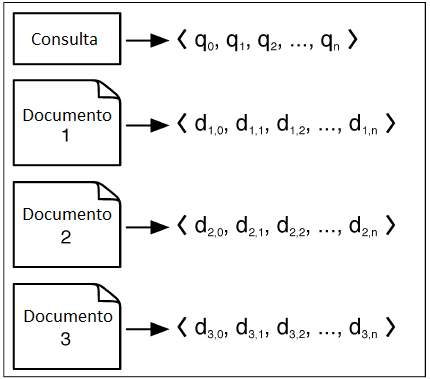
\includegraphics[scale=1.0]{chapters/informationretrieval/Document_as_Vectors.png}
	\caption{Representação dos vetores do modelo de espaço vetorial \citep{Grossman2004}.}
	\label{fig:documento-vetor}
\end{figure}

Este modelo envolve a construção de um vetor que representa os termos de um documento e outro vetor que representa os termos da pesquisa. Em seguida, um método de avaliação deve ser escolhido para medir o grau de aproximação de qualquer vetor documento com o vetor da consulta. Pode-se avaliar a diferença entre a magnitude entre dois vetores, mas geralmente isso prejudica documentos muito grandes e pode dar vantagem para documentos pequenos mas que não possuem muita similaridade \citep{Croft2010}.

Para continuar o entendimento sobre a similaridade desse modelo, é importante alguns conceitos sobre frequência de termos, frequência em documentos e frequência em coleção de documentos que serão abordados em seguida.

\subsection{Frequência de Termos}

De acordo com \cite{Manning2008}, um documento que menciona um termo da consulta mais frequentemente, pode ter uma relação maior com a consulta e, portanto, deveria receber uma pontuação maior. Veremos mais adiante que essa afirmação pode não ser verdade para todos os casos.

Tratando-se de frequência de termos bruta, atribuímos a cada termo de um documento um peso que depende do número de ocorrências do termo no documento. Gostaríamos calcular uma pontuação entre um termo da consulta \textit{t} e um documento \textit{d}, com base no peso de \textit{t} em \textit{d}. A abordagem mais simples é atribuir o peso igual ao número de ocorrências de um termo t num documento d. Este esquema de ponderação é referido como Frequência de Termos e é denotado por \textit{tf\textsubscript{t,d}} \citep{Manning2008}.

A ordem no qual os termos aparecem nos documentos não são levadas em consideração. O importante é apenas reter a frequência total dos termos da busca presentes em cada documento. Essa abordagem é conhecida na literatura como \textit{bag of word} \citep{Croft2010}.

\cite{Manning2008} esclarece ainda, que a frequência bruta não garante que um documento que possua um termo citado 20 vezes é mais relevante do que um documento que possui esse mesmo termo citado dez. Isso porque a relevância não aumenta linearmente proporcional à frequência de termos. Deste modo, frequência de termo logarítmica é mais interessante.

\begin{equation}
w_{t,d} = 
\left\{\begin{matrix}
 &1 +  \log_{10}tf_{t,d},  &se\ tf_{t,d} > 0 \\ 
 &0,  &caso\ contrario 
\end{matrix}\right.
\label{eq:log-tf}
\end{equation}

A tabela seguinte exibe um exemplificação da aplicação da frequência logarítmica de um mesmo termo presente em cinco documentos.

\begin{table}[H]
	\centering
	\caption{Exemplo de aplicação de frequência logarítmica de termos.}
	\label{tab:log-tf-table}
	\def\arraystretch{1.2} % padding da linhas da tabela
	\begin{tabular}{|m{3cm} | m{3cm} | m{3cm} |}

		\hline
		
		\multicolumn{1}{|c|}{\bfseries Documento } & \multicolumn{1}{c|}{\bfseries Frequência} & \multicolumn{1}{c|}{\bfseries Frequência log.}\\ \hline
		d1   					&	0		&	0 	\\ \hline
		d2   					&	1		&	1 	\\ \hline
		d3   					&	2		&	1,3 \\ \hline
		d4   					&	10		&	2	\\ \hline
		d5   					&	1000	&	4 	\\ \hline
		
	\end{tabular}
\end{table}

Como pode ser observado, ainda há importância na quantidade de ocorrência do termo, mas essa frequência não é mais tão determinante na relevância já que a frequência logarítmica aproxima os documentos.

\subsection{Frequência Inversa em Documentos}

 A utilização da frequência inversa em documentos vem da ideia de que termos mais raros são semanticamente mais informativos do que termos comuns. Termos comuns geralmente não possuem o poder de determinar o conteúdo de um documento, mas a presença de um termo raro em um documento aumenta a probabilidade deste documento ser estar fortemente relacionado à ele e, consequentemente, mais relevante para a busca \citep{Manning2008}.

Por exemplo, na área de Ciência da Computação, os termos \textit{código} e \textit{algoritmo} estão muito presentes nos mais diversos tipos de documentos. Se um usuário buscar por \textit{algoritmo de Dijkstra} e o sistema der importância igual aos dois termos e buscar por documentos que possuam apenas o termo \textit{algoritmo}, é improvável que esses documentos satisfaçam o usuário. Neste exemplo, o termo \textit{Dijkstra} tem o valor muito mais determinante na busca do que \textit{algoritmo} e, portanto, deve ter um peso maior na escolha dos documentos.

A definição trazida por \cite{Manning2008} diz que a frequência de documentos \textit{df\textsubscript{t}} corresponde ao total de documentos em uma coleção que contém o termo \textit{t} buscado. Disso, a frequência inversa em documentos, é a medida inversa da informatividade de um termo \textit{t}. Ou seja, quanto menor a frequência de documentos que no qual o termo \textit{t} está presente de uma dada coleção de documentos, mais informativo esses documentos devem ser. Essa fórmula é definida por:

\begin{equation}
idf = \log_{10}(N/df_{t})
\label{eq:idf}
\end{equation}

\subsection{TF–IDF}

Com essas duas medidas definidas acima, Frequência de Termos e Frequência Inversa em Documentos, pode-se aplicar \textit{tf-Idf weight} para determinar a importância do termo presente no documento com relação à coleção total de documentos. Em linhas gerais, tf-idf weight aumenta de acordo com o número de ocorrências de um termo e um documento e também aumenta de acordo com a raridade dos termos presentes no mesmo documento \cite{Manning2008}. 

Tf-idf possui três esquemas mas para simplificação e objetivo deste trabalho, abordaremos apenas a seguinte:
 
\begin{equation}
w_{t,d} = (1 + \log tf_{t,d}) \cdot \log_{10}(N/df_{t})
\label{eq:tf-idf}
\end{equation}

\subsection{Okapi BM25}

\section{Métodos de avaliação}
A partir das opções disponibilizadas para construir sistemas de recuperação da informação, resta buscar meios para os avaliar. Considerando que não existe método perfeito para todos os problemas é necessário se conduzir uma pesquisa para averiguar-se qual a melhor solução para determinado problema. Para fazer isso, determinam-se métricas que irão indicar se há conformidade da solução com o problema.

Uma das formas de se executar um experimento para avaliar o sistema é utilizar um conjunto de buscas e seus resultados esperados. A partir dessas buscas, avaliam-se as condições com que foram apresentados os resultados, levando em consideração desde o tempo que custou para achar essas informações até a quantidade de esforço necessária do usuário para encontrar uma informação relevante dentro do conjunto de resultados. Sendo estas as principais condições:
%As métricas mais relevantes podem variar de problema para problema, já que em alguns podemos ter algumas restrições que outros não possuam, como tempo, por exemplo
\begin{itemize}
    \item \textbf{Cobertura}. Representa o quanto de informações relevantes foram apresentadas como resultados. Considerando que para uma busca X existam 10 resultados relevantes, se apenas 3 foram apresentados para o usuário, temos uma cobertura de 30\%.
    \item \textbf{Ranking}. Métricas que utilizam o rank como parâmetro, avaliam o sistema de acordo com a posição dos itens relevantes nos resultados da busca. Um exemplo deste é o Mean Reciprocal Rank, onde para cada busca, a posição do primeiro documento relevante chamada K é usada pra determinar o Reciprocal Rank que é 1/K, em seguida, deve-se continuar executando mais N buscas onde encontraremos a média desses valores a partir de (1/K1 + 1/K2 + ... )/ N para encontrar o Mean Reciprocal Rank.
    \item \textbf{Precisão}. Informa o quanto de conteúdo relevante existe dentre os documentos apresentados. Por exemplo, se dentre 10 resultados retornados, apenas 2 resultados forem relevantes, temos uma precisão de 20\%.
    \item \textbf{Tempo de resposta}. É o intervalo médio entre o momento da consulta e a apresentação dos resultados.
    \item \textbf{Esforço do usuário}. Representa o esforço despendido pelo usuário para obter resultados em sua busca. Isso pode incluir diversos fatores que variam de acordo com a especificação do problema, sendo exemplos deles: número de linhas lida, número de ações necessárias para executar a busca, número de documentos abertos até encontrar o resultado desejado e outros.
\end{itemize}

\section{Tecnologias e Frameworks}

Para melhor lidar com os desafios de Recuperação da Informação, foram criadas novas tecnologias e frameworks. Essas tecnologias implementam os conceitos aqui utilizados e permitem modificações para que se adaptem melhor ao problema em questão. Os seguintes frameworks são os mais populares.

\begin{itemize}
    \item \textbf{Lucene}. O Apache Lucene é um motor de busca escrito em Java com ferramentas para busca em texto. É uma API open source disponível para download gratuito. Possui uma linguagem própria que permite fazer buscas parametrizadas com expressões regulares. 
    \item \textbf{Solr}. Solr é uma aplicação web construída ao redor do Lucene que adiciona funcionalidades como: busca geospacial, replicação, cacheamento e interfaces de administração.
    \item \textbf{Elasticsearch}. Assim como Solr, o Elasticsearch é uma aplicação construída com o uso do Lucene. O Elasticsearch é distribuído pela empresa Elastic e possui diversos plugins gratuitos e pagos para adicionar-se ferramentas de administração. Diferencia-se do Solr por focar mais em aspectos da administração do banco de dados e na escalabilidade.
\end{itemize}

\section{Sumário}

Foi abordado neste capítulo como e onde a Recuperação Informação é utilizada. Foi tratada a diferença entre Recuperação de Informação e Recuperação Dados e abordada algumas estratégias na recuperação de informações e como as avaliar. Houve um aprofundamento em modelos vetoriais, método que será usado neste trabalho.
\chapter{Proposta}
\label{cap:project}

\begin{quotation}[]{Yoko Ono}
The computer is my favourite invention. I feel lucky to be part of the global village. I don't mean to brag, but I'm so fast with technology. People think it all seems too much, but we'll get used to it. I'm sure it all seemed too much when we were learning to walk.
\end{quotation}

Com o objetivo de facilitar o acesso de usuários à fóruns, este trabalho traz como proposta um buscador que além de tratar a similaridade semântica, também leva em consideração a opinião da comunidade.
\section{Arquitetura}
% Todo usar figuras genéricas
%TODO Migração puxar de base de dados e envia para engenho de busca.
\begin{figure}[htb]
	\centering
	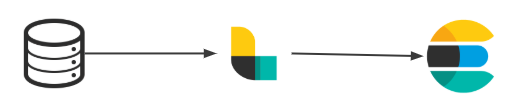
\includegraphics[width=\textwidth]{chapters/project/architecture.png}
	\caption{Arquitetura do sistema proposto}
\end{figure}
Neste projeto, será considerada uma arquitetura plugável à uma base pré-existente, a fim de manter a implantação do sistema o mais simples possível para que outros também possam o implementar em seus fóruns pré-existentes. 
A partir da base já existente do fórum, deve-se ter um serviço que trabalhe de forma contínua extraindo os dados e populando o engenho de buscas. O pré-processamento pode ser realizado tanto no serviço de migração ou no próprio engenho de busca. Entretanto, é essencial que o engenho de busca seja capaz de indexar e recuperar os dados armazenado de forma eficiente, conforme descrito nesse capítulo.

\section{Modelo Entidade Relacionamento}
\label{mer}

\begin{figure}[htb]
	\centering
	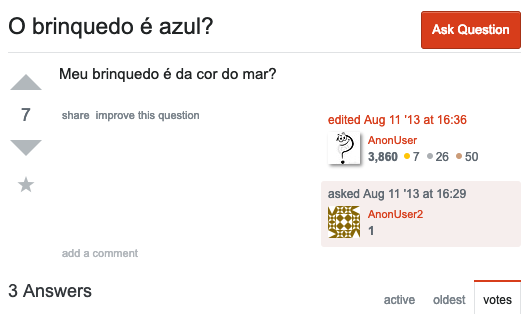
\includegraphics[width=\textwidth]{chapters/project/question-brinquedo.png}
	\caption{Exemplo de tópico}
	\label{fig:screenshootquestion}
	% TODO Verificar referências ao AskUbuntu
\end{figure}
Nos fóruns observados, foi percebido que os tópicos podem ter tanto título e corpo. Entende-se como corpo, o conteúdo textual descritivo da primeira postagem. Ao permitir que usuários votem indicado a utilidade ou qualidade de um documento, é adicionado um conceito de pontuação. Fóruns que não implementam recursos de avaliação, podem usar outros parâmetros para definir a pontuação de um documento, como número de visualizações ou alguma outra métrica de engajamento, por exemplo.

\begin{figure}[htb]
	\centering
	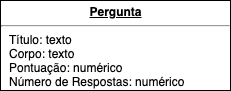
\includegraphics[scale=1.0]{chapters/project/mer.png}
	\caption{Formato exigido}
\end{figure}

\section{Pré-processamento}
Cada tópico passará por transformações antes de serem armazenadas. Considere os títulos descritas na tabela \ref{tab:example} no seu estado inicial. Estes irão ilustrar o pré-processamento. Vale ressaltar que o mesmo processo que está sendo descrito com os títulos também ocorre com o corpo.

\begin{table}[htb]
	\centering
    \def\arraystretch{1.2} % padding da linhas da tabela
    \begin{tabular}{|l|l|}
        \hline
        1 & <p>I will organize this room</p>            \\ \hline
        2 & All rooms are organized and clean \\ \hline
        3 & Cleaners are <b>very</b> effective                              \\ \hline
        4 & I will open this window                            \\ \hline
    \end{tabular}
	\caption{Frases de exemplo}
    \label{tab:example}
\end{table}


\subsection{Filtros de caracteres}
Na web é comum encontrar documentos com tags HTML. Para este projeto, estas tags não terão importância, portanto serão removidas e apenas será deixado apenas o texto. É possível verificar o resultado exemplificado na tabela \ref{tab:charfilter}.

\begin{table}[htb]
	\centering
    \def\arraystretch{1.2} % padding da linhas da tabela
    \begin{tabular}{|l|l|l|}
        \hline
        & \textbf{Antes} & \textbf{Depois} \\ \hline
        1 & <p>I will organize this room</p> & I will organize this room            \\ \hline
        2 & All rooms are organized and clean & All rooms are organized and clean \\ \hline
        3 & Cleaners are <b>very</b> effective & Cleaners are very effective                              \\ \hline
        4 & I will open this window & I will open this window                             \\ \hline
    \end{tabular}
	\caption{Frases de exemplo após os filtros de caracteres}
    \label{tab:charfilter}
\end{table}

\subsection{Tokenização}
O processo de tokenização é responsável por dividir um texto em unidades menores. Essas unidades podem ser palavras, caracteres, cadeia de palavras ou cadeia de caracteres. 

Para este projeto, foi usado a tokenização dividindo o conteúdo do texto em palavras usando o algoritmo Unicode Text Segmentation \cite{unicodesegmentation}.

\begin{table}[htb]
	\centering
    \def\arraystretch{1.2} % padding da linhas da tabela
    \begin{tabular}{|l|l|l|}
        \hline
        & \textbf{Antes} & \textbf{Depois} \\ \hline
        1 & I will organize this room & [I, will, organize, this, room]            \\ \hline
        2 & All rooms are organized and clean & [All, rooms, are, organized, and, clean] \\ \hline
        3 & Cleaners are very effective & [Cleaners, are, very, effective]                              \\ \hline
        4 & I will open this window & [I, will, open, this, window]                             \\ \hline
    \end{tabular}
	\caption{Frases de exemplo após a tokenização}
    \label{tab:tokenization}
\end{table}

\subsection{Transformações}
Algumas transformações podem se fazer necessárias no corpus. Foi usada nesse projeto uma transformação responsável por deixar todos os caracteres minúsculos.

\begin{table}[htb]
	\centering
    \def\arraystretch{1.2} % padding da linhas da tabela
    \begin{tabular}{|l|l|l|}
        \hline
        & \textbf{Antes} & \textbf{Depois} \\ \hline
        1 & [I, will, organize, this, room] & [i, will, organize, this, room]            \\ \hline
        2 & [All, rooms, are, organized, and, clean] & [all, rooms, are, organized, and, clean] \\ \hline
        3 & [Cleaners, are, very, effective] & [cleaners, are, very, effective]                              \\ \hline
        4 & [I, will, open, this, window] & [i, will, open, this, window]                             \\ \hline
    \end{tabular}
	\caption{Frases de exemplo após as transformações}
    \label{tab:transformations}
\end{table}

\subsection{Filtros de tokens}
\subsubsection{Remoção de Stop Words}
Existem palavras que adicionam pouco valor semântico ao texto, são conhecidas como \textit{stop words}. Stop words são palavras como: isso, um, a, o, que. Estas também serão removidas. Existem diversas formas de as detectar em um corpus, as mais comuns são com uso de listas com stop words predefinidas ou definindo um limiar máximo de ocorrências que uma palavra pode ter. Assume-se que palavras que ocorrem frequentemente em vários documentos não agregam muito conteúdo ao texto.

\begin{table}[htb]
	\centering
    \def\arraystretch{1.2} % padding da linhas da tabela
    \begin{tabular}{|l|l|l|}
        \hline
        & \textbf{Antes} & \textbf{Depois} \\ \hline
        1 & [i, will, organize, this, room] & [organize, room]            \\ \hline
        2 & [all, rooms, are, organized, and, clean] & [rooms, organized, clean] \\ \hline
        3 & [cleaners, are, very, effective] & [cleaners, effective]                              \\ \hline
        4 & [i, will, open, this, window] & [open, window]                             \\ \hline
    \end{tabular}
	\caption{Frases de exemplo após a remoção de stop words}
    \label{tab:tokenfilter}
\end{table}

\subsubsection{Stemming}
O propósito do stemming é reduzir a variação morfológica das palavras \cite{stemmingdef}. Documentos podem usar formas diferentes de uma palavra, por exemplo, um deles pode usar organizar, outro pode usar organizando e outro organizado. Embora as palavras não sejam idênticas, elas trazem consigo um sentido similar, o que pode ser útil em um sistema de recuperação da informação onde se deseja conteúdo relacionado, ainda que não idêntico.

\begin{figure}[htb]
	\centering
	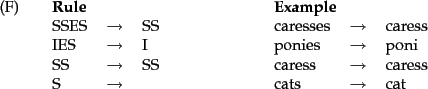
\includegraphics[width=\textwidth]{chapters/project/porterrules.png}
	\caption{Regras usadas na primeira fase do Porter Stemmer}
    \label{fig:porterstemmerprocess}
\end{figure}

O algoritmo mais comum de Stemming é o Porter \cite{porterstemming}. Este algoritmo usa fases com conjuntos definidos de regras para definir as transformações que uma dada palavra irá passar. A figura \ref{fig:porterstemmerprocess} mostra algumas das regras executadas na primeira fase do algoritmo.

Pode-se ver que agora, que as frases descritas na tabela \ref{tab:tokenfilter}, possuem mais palavras em comum do que anteriormente, isso garante uma busca mais abrangente, permitindo o usuário ter resultados com palavras diferentes da sua, mas que ainda acessem o mesmo domínio. Entretanto o resultado não é perfeito, palavras relacionadas podem acabar tendo finais diferentes e palavras diferentes podem possuir o mesmo resultado.
\begin{table}[htb]
	\centering
    \def\arraystretch{1.2}
    \begin{tabular}{|l|l|l|}
        \hline
        & \textbf{Antes} & \textbf{Depois} \\ \hline
        1 & [organize, room]  & [organ, room]            \\ \hline
        2 & [rooms, organized, clean]  & [room, organ, clean] \\ \hline
        3 & [cleaners, effective]  & [cleaner, effect]                              \\ \hline
        4 & [open, window]  & [open, window]                             \\ \hline
    \end{tabular}
	\caption{Frases de exemplo após o stemming}
    \label{tab:tokenfilter}
\end{table}

\subsection{Sumário}
Percebe-se na tabela \ref{tab:allphrases} o quanto cada uma das frases mudou e agora é possível verificar alguns padrões se repetindo onde não seria tão fácil se identificar previamente.
\begin{table}[htb]
	\centering
    \def\arraystretch{1.2} % padding da linhas da tabela
    \begin{tabular}{|l|l|l|}
        \hline
        & \textbf{Incial} & \textbf{Final} \\ \hline
        1 & <p>I will organize this room</p>  & [organ, room]            \\ \hline
        2 & All rooms are organized and clean  & [room, organ, clean] \\ \hline
        3 & Cleaners are <b>very</b> effective  & [cleaner, effect]                              \\ \hline
        4 & I will open this window  & [open, window]                             \\ \hline
    \end{tabular}
	\caption{Frases de exemplo ao final do pré-processamento}
    \label{tab:allphrases}
\end{table}

 Na tabela \ref{tab:quenstionpreprocessed} percebe-se o mesmo processo aplicado aos campos título e corpo de um tópico.

\begin{table}[htb]
	\centering
    \def\arraystretch{1.2} % padding da linhas da tabela
    \begin{tabular}{|l|l|l|}
        \hline
        & \textbf{Inicial} & \textbf{Final} \\ \hline
        \textbf{Título}              & O brinquedo é azul?            & [brinq, azul] \\ \hline
        \textbf{Descrição}               & Meu brinquedo é da cor do mar? & [brinq, cor, mar] \\ \hline
        \textbf{Pontuação}           & 7                              & 7 \\ \hline
    \end{tabular}
	\caption{Tópico após o pré-processamento}
    \label{tab:quenstionpreprocessed}
\end{table}     
\section{Indexação e Recuperação}
Concluído o pré-processamento, deve-se armazenar estes documentos, de forma que seja possível os recuperar em outro momento. Entretanto, métodos comuns encontrados na maioria dos bancos de dados são inadequados para lidar com texto.

Índices invertidos foram criados para serem uma forma rápida para lidar com dados massivos de texto. Para cada termo, é salvo o número de ocorrências e em que documentos eles ocorrem, conforme descrito na tabela \ref{tab:invertedindex}. Para cada campo de um tópico, existe um índice, ou seja, além do índice dos títulos na tabela \ref{tab:invertedindex}, ao realizar o pré-processamento do corpo, também haverá um índice para os corpos. 

\begin{table}[htb]
	\centering
    \def\arraystretch{1.2} 
    \begin{tabular}{|l|l|l|}
        \hline
        \textbf{Termo} & \textbf{Frequência} & \textbf{Documentos} \\ \hline
        organ & 2  & 1, 2            \\ \hline
        room & 1  & 2 \\ \hline
        clean & 1  & 2                              \\ \hline
        cleaner & 1  & 3                             \\ \hline
        effect & 1  & 3                             \\ \hline
        open & 1  & 4                             \\ \hline
        window & 1  & 4                             \\ \hline
    \end{tabular}
	\caption{Frases de exemplo no índice invertido}
    \label{tab:invertedindex}
\end{table}
Ao executar uma busca, o texto informado pelo usuário passa pelo mesmo processo de preprocessamento. Dessa forma, os tokens gerados ao final do pré-processamento serão usados para encontrar resultados na base que possuam um ou mais tokens em comum. Estes índices serão usados para também otimizar o processo de ranking, que o usará para avaliar a relevância de cada um dos termos.

\section{Ranking}
Na seção anterior, foi explicado como encontrar documentos relacionados. Nesta seção será explicado como definir a prioridade entre os selecionados, ou seja, determinar quais devem aparecer primeiro.

Será usado o algoritmo Okapi BM25, descrito no capítulo \ref{cap:informationretrieval}. Com o uso somente do cálculo de similaridade, já é possível ordenar os resultados. Entretanto, o Okapi BM25 não leva em consideração a pontuação adquirida pelo tópico, o que causa grandes impactos no resultado como será visto no capítulo \ref{cap:evaluation}. Devido à isso, é definida a relevância \textit{Rel} de um tópico \textit{x} para uma busca \textit{b} é definido pela média dos valores de similaridades obtidos pela função \textit{sim} da busca com título \textit{t} e da busca com corpo \textit{c} multiplicados com a pontuação \textit{p} obtida pelo tópico. Além disso, também é definido um parâmetro \textit{i} para regular a influência da similaridade no cálculo. Este cálculo é formalmente apresentado na equação \ref{eq:rel} e na tabela \ref{tab:relevance} é exemplificado o processo de ranking com dados fictícios.

\begin{equation}
    Rel(q, x) = \left(\frac{sim(t_{x}, b)  sim(c_{x}, b)}{2}\right)^{i}  p_{x} 
    \label{eq:rel}
\end{equation}

\begin{table}[htb]
	\centering
    \def\arraystretch{1.2} % padding da linhas da tabela
    \begin{tabular}{|l|l|l|l|l|}
        \hline
        Tópico & Sim. Título & Sim. Corpo & Pontuação & \textbf{Relevância} \\ \hline
        1 & 3 & 11 & 7 & 102487 \\ \hline
        2 & 0 & 1 & 1600 & 100 \\ \hline
        3 & 0 & 0 & 327 & 0 \\ \hline
        4 & 4 & 4 & 80 & 20480 \\ \hline
    \end{tabular}
	\caption{Cálculo de relevância das frases de exemplo. \textit{i} = 4}
    \label{tab:relevance}
\end{table}


\section{Tecnologias Utilizadas}
Para tornar essa aplicação real, foi usado um conjunto de ferramentas que auxiliam os processos descritos anteriormente nesse capítulo.
\begin{itemize}
    \item \textbf{Elasticsearch}. Este engenho de busca, já mencionado no capítulo \ref{cap:informationretrieval} foi configurado para trabalhar com fóruns. O Elasticsearch\footnote{https://www.elastic.co/products/elasticsearch} foi criado pela empresa Elastic\footnote{https://www.elastic.co/} e é uma ferramenta open source e gratuita, ainda que pertença à uma empresa privada. Ele pode ser configurado com diferentes plugins que interagem desde o processo de indexação até a sua administração. É o engenho de busca mais popular do mercado devido suas ferramentas empresariais, frequentemente usado para hospedar os logs dos sistemas. Já funciona como serviço na AWS\footnote{https://aws.amazon.com/} e no GCP\footnote{https://cloud.google.com/}.
    \item \textbf{Logstash}. Criado inicialmente com o objetivo de tratar os logs das aplicações, o Logstash\footnote{https://www.elastic.co/products/logstash} é uma ferramenta produzida também pela Elastic. O mesmo é capaz de extrair diversas informações de fontes de dados, atualmente não só mais de logs, mas também de bancos de dados, arquivos, páginas web e outros, tratar esses dados com operações desde simples regex até complexos joins em sistemas de banco de dados para, enfim, os salvar em uma outra localidade, que pode ser um arquivo ou, mais comumente utilizado, no Elasticsearch. Foi usado para migrar os dados do banco de dados para o Elasticsearch.
    \item \textbf{Kibana}. Para finalizar, o Kibana\footnote{https://www.elastic.co/products/kibana} é o último participante do grupo \acs{ELK}. Esta é uma ferramenta também produzida pela empresa Elastic que cuida de visualização de dados com suporte a linguagem Lucene\footnote{http://lucene.apache.org/}. Esta também é capaz de monitorar o Elasticsearch através do seu \ac{APM} e gerar visualizações a partir disso. Conta com um painel de gerenciamento do Elasticsearch para realizar operações críticas e não-críticas e também com um espaço para realizar benchmarks e testes de operações específicas.
    \item \textbf{MySQL}. O banco de dados MySQL\footnote{https://www.mysql.com/} é um dos mais populares bancos relacionais existentes. Neste projeto, ele foi responsável por manter a base de dados organizada, e também por representar um fórum já existente com uma base própria. Suas funcionalidades permitiram uma rápida iteração no projeto, graças à facilidade de extrair novas informações ao mudar os requisitos. Este banco de dados também conta com estruturas de índices, que garantiu que as migrações fossem feitas rapidamente. Sua robustez e tempo de existência fazem diferença, possui estruturas e ferramentas que usam a performance das máquinas para distribuir as cargas de trabalho de forma mais eficiente.
    \item \textbf{Docker}. Docker\footnote{https://docker.com/} é um ambiente de virtualização que faz uso de contêineres. Foi criado com o objetivo de criar ambientes prontos para a produção, onde a configuração de um sistema é definida em um arquivo chamado Dockerfile e, ao ser executado, configura um contâiner com as definições impostas. É uma opção que tem sido considerada a sucessora ao de uso de máquinas virtuais, pois usa uma tecnologia que garante o isolamento com o resto do sistema sem comprometer tanto a performance. Neste projeto, foi usado para rapidamente ter acesso às outras tecnologias descritas aqui e poder construir e reconstruir ambientes de forma simples.
    \item \textbf{Python}. Esta linguagem de programação, é comumente usada para aplicações de \ac{RI} e de \ac{NLP}, graças à um grande número de bibliotecas, como NLTK\footnote{https://www.nltk.org/}, Scikit-learn\footnote{https://scikit-learn.org/}, Pandas\footnote{https://pandas.pydata.org/}, NumPy\footnote{http://www.numpy.org/} e outras, além de uma comunidade participativa. Python\footnote{https://www.python.org/} foi criada em 1991 e tem sido usada em projetos de diferentes tipos, é extremamente popular e considerada uma linguagem fácil para estudantes aprenderem como primeira linguagem de programação. A linguagem foi utilizada para a realização de buscas, testes e análises nesta pesquisa.
\end{itemize}
\section{Sumário}

\chapter{Avaliação}
\label{cap:evaluation}

\begin{quotation}[]{Yoko Ono}
The computer is my favourite invention. I feel lucky to be part of the global village. I don't mean to brag, but I'm so fast with technology. People think it all seems too much, but we'll get used to it. I'm sure it all seemed too much when we were learning to walk.
\end{quotation}

\section{Metodologia}
\section{Conjunto de Dados}
\section{Métricas de Avaliação}
\section{Resultados}
\section{Discussão}
\section{Sumário}
\chapter{Conclusão}
\label{cap:conclusion}

\begin{quotation}[]{Yoko Ono}
The computer is my favourite invention. I feel lucky to be part of the global village. I don't mean to brag, but I'm so fast with technology. People think it all seems too much, but we'll get used to it. I'm sure it all seemed too much when we were learning to walk.
\end{quotation}

\section{Contribuições}
\section{Pontos de melhorias}
\section{Trabalhos Futuros}
\section{Sumário}

\bibliographystyle{natbib}
\addcontentsline{toc}{chapter}{\bibliographytocname}
\bibliography{references}

% Appendix
%\clearpage
%\addappheadtotoc
%\appendix
%\appendixpage
%\chapter{Formulário}
\label{ap:formulario}


\def \tick{
$[$\hspace{0.3cm}$]$
}

\def \twooption#1#2{
\tick #1.  \tick #2.
}

\def \threeoption#1#2#3{
\tick #1.\newline
\tick #2.\newline
\tick #3.
}

\def \fouroption#1#2#3#4{
\tick #1.\newline
\tick #2.\newline
\tick #3.\newline
\tick #4.
}

\def \fiveoption#1#2#3#4#5{
\tick #1.\newline
\tick #2.\newline
\tick #3.\newline
\tick #4.\newline
\tick #5.
}
\def \datefield{
%date fied used in time sheets
    /\hspace{0.4cm}/
}

\def \rcolor{
%table row color
    \rowcolor[gray]{0.9}
}

\def \hcolor{
    \rowcolor[gray]{0.7}
}


\section{Formulário para o usuário do NLP Discovery}
\label{ap:sec:feedback}

\textbf{Nome: }
\\
\line(1,0){380}
\\
\textbf{Você tem algum conhecimento técnico a respeito de Serviços Web? }
\\
\twooption{Sim}{Não}
\\
\textbf{Encontrou alguma dificuldade ao utilizar a ferramenta?}
\\
\twooption{Sim}{Não}
\\
\textbf{Caso tenha respondido "Sim", detalhe a dificuldade encontrada:}
\\
\line(1,0){410}
\\
\line(1,0){410}
\\
\line(1,0){410}
\\
\line(1,0){410}
\\
\textbf{Qual foi a consulta realizada na ferramenta (Digite exatamente o mesmo texto que digitou na caixa de pesquisa da ferramenta)?  }
\\
\line(1,0){410}
\\
\line(1,0){410}
\\
\line(1,0){410}
\\
\line(1,0){410}
\\
\textbf{A busca gerou algum resultado relevante?}
\\
\twooption{Sim}{Não}
\\
\textbf{Caso tenha respondido "Sim", qual a posição do Serviço relevante no resultado?}
\\
\line(1,0){100}
\\


\end{document}
